\section{Προσομοίωση}
Το κυκλώματα με τις τιμές των παραμέτρων του πίνακα \ref{table:estimate}, όταν προσομοιώθηκε, δεν πληρούσε την προδιαγραφές για gain-bandwidth product και το περιθώριο φάσης. Το κέρδος ανοιχτού βρόχου πληρεί την προδιαγραφή του πίνακα \ref{table:specs}.\par

\subsection{Ρυθμίσεις}
Το κέρδος τάσης ανοιχτού βρόχου δίνεται από την έκφραση
\begin{equation}
	\label{eq:Av}
	A_v=\frac{2\cdot g_{m1}\cdot g_{m6}}{I_{D5}\(\lambda_2+\lambda_5\)\cdot I_{D6}\(\lambda_6+\lambda_7\)}.
\end{equation}

Επιπλέον, για το διαφορικό ζεύγος απαιτείται υψηλή διαγωγιμότητα προκειμένου να μειώνεται η συνεισφορά του θερμικού θορύβου,\cite{lectureSlides} οπότε αυξάνονται οι λόγοι $S_1$ και $S_2$. Αυτό οδηγεί σε μία αύξηση του κέρδους ανοιχτού βρόχου, παρόλο που ήταν ήδη εντός των προδιαγραφών.

Το gain-bandwidth product δίνεται από την έκφραση
\begin{equation}
	\mathrm{GB}=A_v(0)\cdot|\omega_{p_1}|=\frac{g_{m1}}{C_C}.
\end{equation}
Αυτό σημαίνει πως η αύξηση των $S_1$ και $S_2$ βελτιώνει και το gain-bandwidth το οποίο επιβεβαιώνεται και από το την προσομοίωση. Τα $g_{m1}$, $g_{m2}$ μπορούν να αυξηθούν και μέσω της αύξησης του $I_{D5}=\sfrac{I_{D1}}{2}$ το οποίο όμως, εξαιτίας της σχέσης \ref{eq:Av}, φαίνεται να μειώνει το κέρδος ανοιχτού βρόχου. To $I_{D5}$ αυξάνεται μέσω της αύξησης του $I_{\mathrm{ref}}$. Με αύξηση του $S_5$ στο δεκαπλάσιο της αρχικής του τιμής, το $I_{D5}$ φαίνεται να δεκαπλασιάζεται και αυτό με αντίκτυπο στο κέρδος ανοιχτού βρόχου το οποίο όμως παραμένει εντός των προδιαγραφών.\par
Επιπλέον, η αύξηση, κατά περίπου $4.4$ φορές, του $S_7$ και κατά συνέπεια του $I_{D7}=I_{D6}$ αν και αναμένεται να μειώσει το κέρδος ανοιχτού βρόχου, έχει μικρή επίδραση σε κλίμακα decibel. Ωστόσο, βελτιώνει σημαντικά το gain-bandwidth product.\par
Το $S_6$ μειώνεται στην μισή τιμή του νέου $S_7$ το οποίο αν και επιδρά αρνητικά στο κέρδος, αυξάνει (προς το μηδέν) την φάση της εξόδου.\par
Η αντίσταση $R_Z$ παίρνει τιμή αρκετά μεγαλύτερη της $\frac{1}{g_{m2}}$ που απαιτείται για την μετατόπιση του μηδενικού σε \textsl{άπειρη} συχνότητα.\cite{sedra} Χρησιμοποιώντας τιμή μεγαλύτερη της $\frac{1}{g_{m2}}$ το μηδενικό μετατοπίζεται στον αρνητικό πραγματικό ημιάξονα και αυξάνει το περιθώριο φάσης.\cite{sedra}\par
Για τη μείωση της κατανάλωσης ισχύος χωρίς να επηρεασθούν σημαντικά οι υπόλοιπες παράμετροι του ενισχυτή, αυξάνεται ελαφρώς, κατά $3\unit{\micro\meter}$, ο λόγος $S_8$.\par
Τέλος, οι λόγοι $S_3$, $S_4$ ρυθμίζονται βάση της σχέσης \eqref{eq:S7a}.\par

Οι προσομοιώσεις έγιναν με το κύκλωμα \ref{circ:op_amp_sim}. Στο κύκλωμα \ref{circ:op_amp_sources} φαίνονται οι πηγές τροφοδοσίας και οι πηγές που εφαρμόζονται στην μη αναστρέφουσα είσοδο για έλεγχο των προδιαγραφών. Η αναστρέφουσα είσοδος συνδέεται μέσω του βρόχου ανάδρασης του κυκλώματος \ref{circ:op_amp_feedback_loop} στην έξοδο του ενισχυτή. \par

\begin{center}
	\begin{circuitfig}[H]
		\centering
		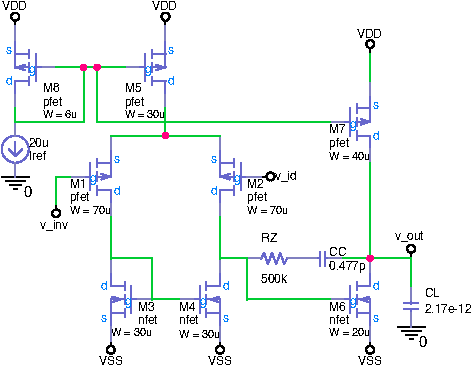
\includegraphics[width=8cm]{op_amp_sim/op_amp_main.pdf}
		\caption{CMOS τελεστικός ενισχυτής δύο σταδίων.Τα μήκη των διαύλων όλων των transistor είναι $L=1\unit{\micro\meter}$ και τα πλάτη αναγράφονται δίπλα στο κάθε transistor.}
		\label{circ:op_amp_sim}
	\end{circuitfig}
	\begin{circuitfig}[H]
		\centering
		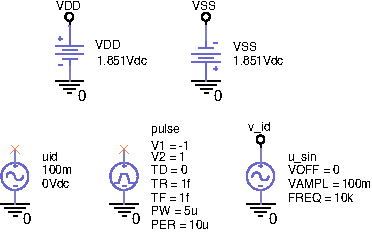
\includegraphics[width=6.3cm]{op_amp_sim/op_amp_sources.pdf}
		\caption{Η πηγή τάσης \texttt{uid} χρησιμοποιείται για την παραγωγή διαγράμματος Bode. Η πηγή \texttt{u\_sin} χρησιμοποιείται στην ανάλυση στο πεδίο του χρόνου (transient analysis) και η πηγή \texttt{pulse} παράγει τετραγωνικό παλμό για την μέτρηση του slew rate.}
		\label{circ:op_amp_sources}
	\end{circuitfig}
	\begin{circuitfig}[H]
		\centering
		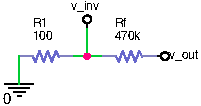
\includegraphics[width=3.5cm]{op_amp_sim/op_amp_feedback_loop.pdf}
		\caption{Δίκτυο ανάδρασης. Η τιμή της $R_f$ δεν μπορεί να είναι πολύ υψηλή διότι θα αυξηθεί η κατανάλωση ισχύος. Λόγω της μεγάλης τιμής της $R_f$ και της μικρής τιμής της $R_1$ η τάση στην αναστρέφουσα είσοδο του τελεστικού είναι πολύ κοντά στη γείωση, της τάξεως λίγων εκατοντάδων $\unit{\micro\volt}$ (κύκλωμα \ref{circ:op_amp_labels}).}
		\label{circ:op_amp_feedback_loop}
	\end{circuitfig}
\end{center}
% \vspace*{-0.5cm}

\subsection{Συχνοτική απόκριση}
% Το κέρδος ανοιχτού βρόχου και η φάση της εξόδου του κυκλώματος \ref{circ:op_amp_schematic} φαίνονται στο διάγραμμα \ref{plot:bode}.

\begin{center}
	\begin{plotenv}[H]
		\centering
		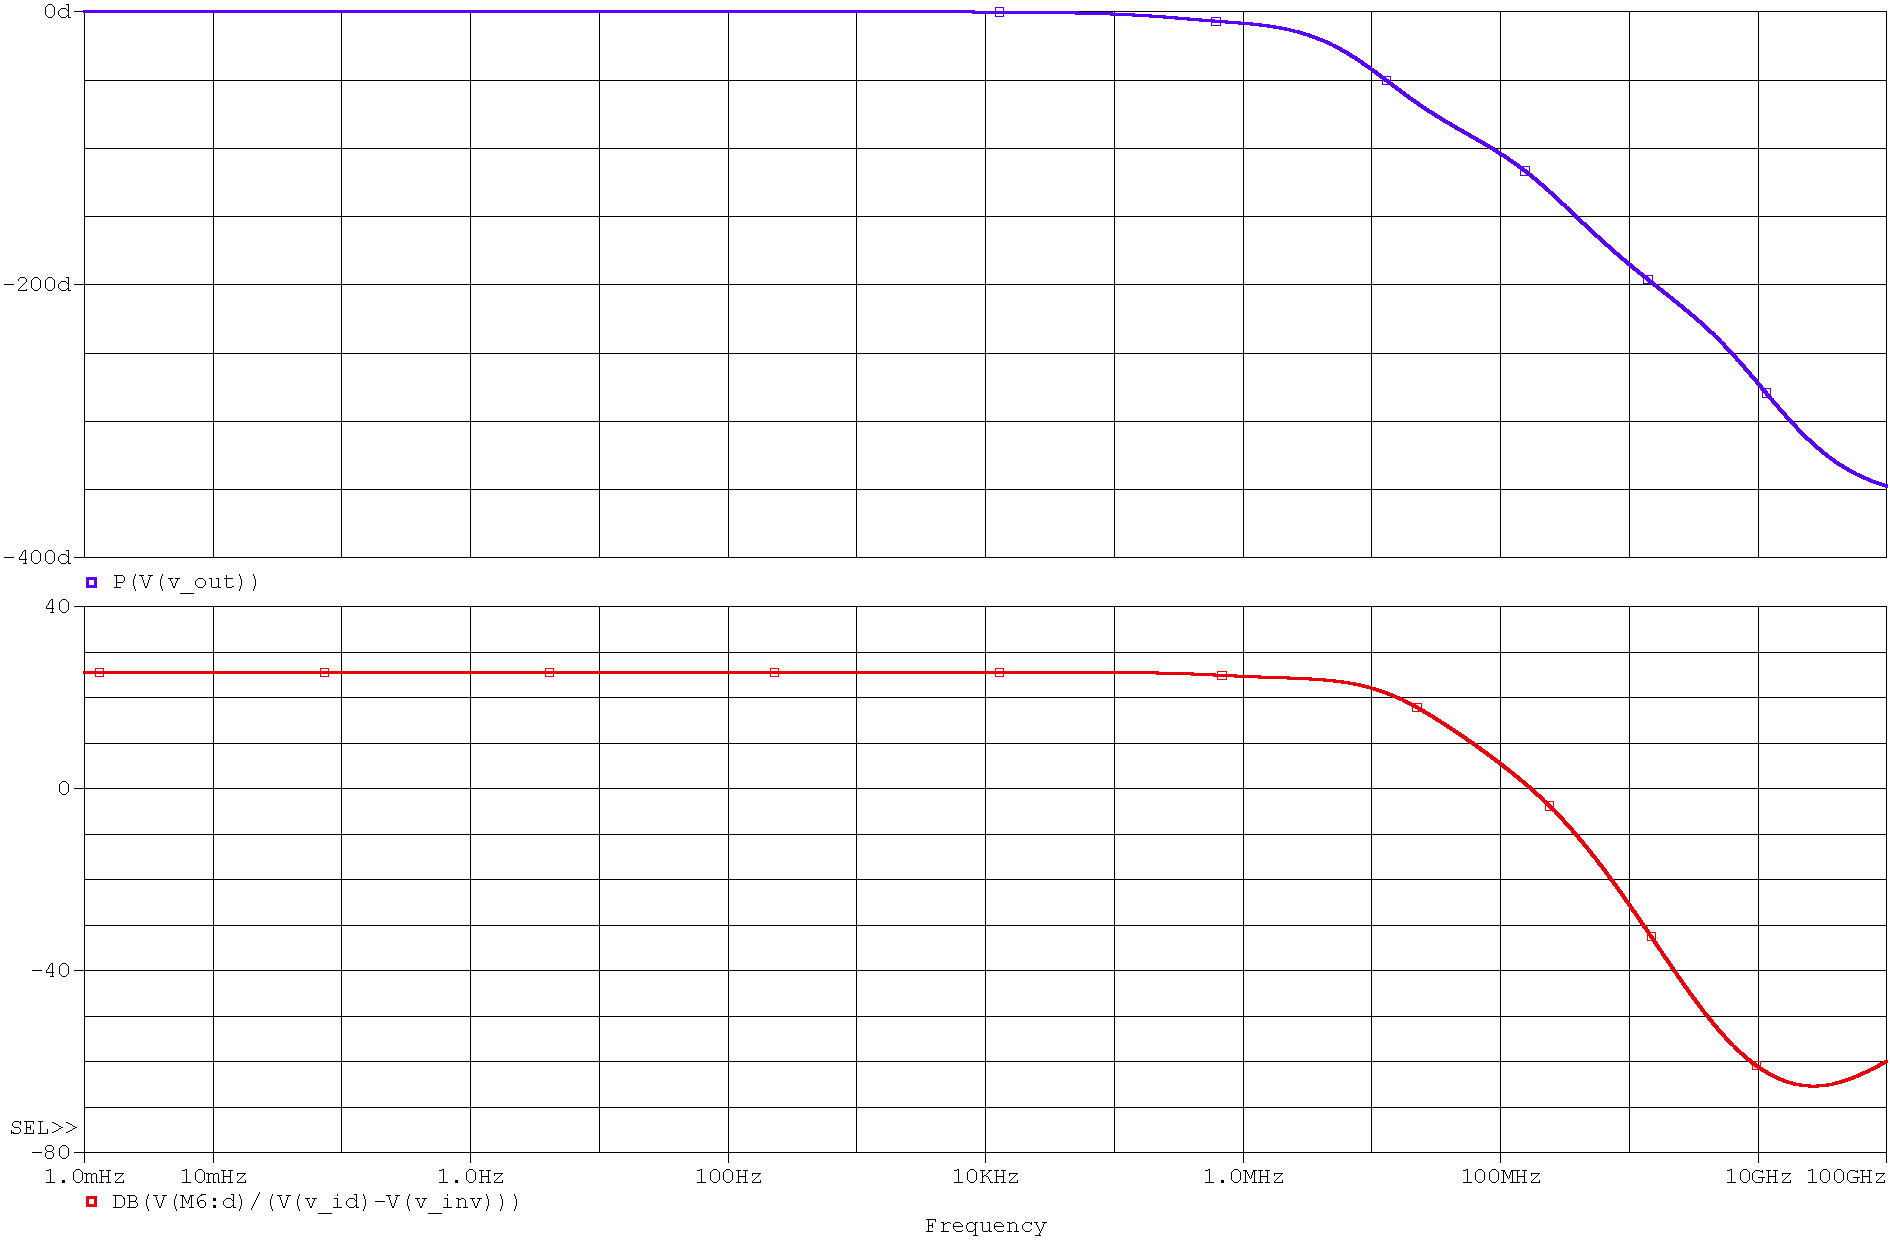
\includegraphics[width=\linewidth]{op_amp_sim/bode.pdf}
		\caption{Με κόκκινο χρώμα διαγράφεται το κέρδος τάσης εξόδου σε $\unit{\decibel}$ και με μπλε χρώμα διαγράφεται η φάση της εξόδου.}
		\label{plot:bode}
	\end{plotenv}
\end{center}
\vspace*{-0.5cm}

Το μέγιστο του κέρδους τάσης στο πεδίο της συχνότητας βρέθηκε στα $20\cdot\log_{10}{A_v}=25.55619$.\par
Το gain-bandwidth product εκτιμήθηκε στο σημείο όπου η καμπύλη του κέρδους σημειώνει μείωση κατά $3\unit{\decibel}$ από την σταθερή τιμή της και βρέθηκε $\mathrm{GB}=8.70313\unit{\mega\hertz}$.\par
Το περιθώριο φάσης βρέθηκε $\phi_M=59.95727^\circ$. Συγκεκριμένα, το περιθώριο φάσης ισούται με το άθροισμα της φάσης της εξόδου στη συχνότητα μοναδιαίου κέρδους (unity gain frequency) και των $180^\circ$.\par
Στον πίνακα \ref{table:gb_measurements} παρατίθενται οι εκφράσεις που χρησιμοποιήθηκαν στο PSpice για τον προσδιορισμό των παραπάνω και το αποτέλεσμά τους.\par
\begin{table}[H]
	\begin{center}
		\begin{tabular}{|c|l|}
			\hline
			\footnotesize{\textbf{Μέγεθος}}                      & \footnotesize{\textbf{PSpice measurement expression}}                        \\\hline\hline
			\tiny{$20\log{(A_v)} \left[\unit{\decibel}\right]$}  & \tiny{\texttt{Max(DB(V(M6:d)/(V(v\_id)-V(v\_inv))))}}                        \\\hline
			\tiny{$\mathrm{GB} \left[\unit{\mega\hertz}\right]$} & \tiny{\texttt{PhaseMargin(DB(V(v\_out)/(V(v\_id)-V(v\_inv))),P(V(v\_out)))}} \\\hline
			\tiny{$\phi_M \left[{}^\circ\right]$}                & \tiny{\texttt{Cutoff\_Lowpass\_3dB(DB(V(v\_out)/(V(v\_id)-V(v\_inv))))}}     \\\hline
		\end{tabular}
		\caption{PSpice measurements για τον υπολογισμό του κέρδους ανοιχτού βρόχου, gain-bandwidth product και του περιθωρίου φάσης της εξόδου.}
		\label{table:gb_measurements}
	\end{center}
\end{table}


\subsection{Κατανάλωση ισχύος}
Η κατανάλωση ισχύος εκτιμάται μέσω transient analysis σε διάστημα μίας περιόδου με ημιτονοειδές σήμα πλάτους $200\unit{\milli\volt}_\mathrm{pp}$ συχνότητας $10\unit{\kilo\hertz}$ συνδεδεμένο στη μη αναστρέφουσα είσοδο του ενισχυτή.\par
Πρώτος τρόπος εκτίμησης είναι μέσω των bias currents του κυκλώματος \ref{circ:op_amp_labels}. Συγκεκριμένα, η κατανάλωση ισχύος θα είναι
\begin{align*}
	P_\mathrm{diss}= & \(|I_{D5}|+|I_{D6}|+|I_{D8}|\)\cdot\(V_{DD}+|V_{SS}|\)                            \\
	=                & \(95.51+144.50+20.00\)\cdot\(1.851+1.851\)\;\unit{\micro\ampere}\cdot\unit{\volt} \\
	=                & 0.963\unit{\milli\watt}\ll 50.17\unit{\milli\watt}.
\end{align*}

\begin{circuitfig}[H]
	\centering
	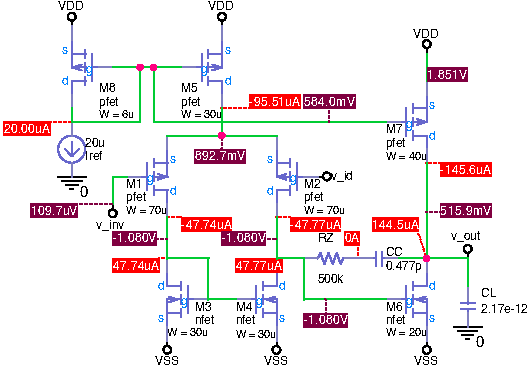
\includegraphics[width=9cm]{op_amp_sim/op_amp_labels.pdf}
	\caption{Bias τάσεις και εντάσεις ρευμάτων για $u_+$ πλάτους $200\unit{\milli\volt}_\mathrm{pp}$ συχνότητας $10\unit{\kilo\hertz}$.}
	\label{circ:op_amp_labels}
\end{circuitfig}

Ο δεύτερος τρόπος είναι η ανάγνωση της τιμής από το output αρχείο της προσομοίωσης, \texttt{trans.out} στην προκειμένη. Ειδικότερα, η κατανάλωση ισχύος είναι $0.928\unit{\milli\watt}$ όπως φαίνεται από το παρακάτω χωρίο του \texttt{trans.out}.\par
\footnotesize{\begin{verbatim}
	VOLTAGE SOURCE CURRENTS
	NAME         CURRENT

	V_uid        0.000E+00
	V_VSS       -2.400E-04
	V_pulse      0.000E+00
	V_VDD       -2.611E-04
	V_u_sin      0.000E+00

	TOTAL POWER DISSIPATION   9.28E-04  WATTS
\end{verbatim}}

\subsection{Slew rate}
Για τον υπολογισμό του slew rate, κατά τις οδηγίες της εκφώνησης, στην μη αναστρέφουσα είσοδο του ενισχυτή εφαρμόσθηκε τετραγωνικός παλμός πλάτους $1\unit{\volt}$. Παρακολουθείται η έξοδος σε θετική ακμή του παλμού της εισόδου. Βρίσκεται η χρονική στιγμή κατά την οποία η έξοδος είναι στο $10\%$ του πλάτους της peak to peak και βρίσκεται και η χρονική στιγμή κατά την οποία η έξοδος είναι στο $90\%$ του πλάτους της peak to peak. Το slew rate θα είναι ο λόγος $\mathrm{SR}=\displaystyle{\frac{u_{0.9}-u_{0.1}}{t_{0.9}-t_{0.1}}}$.\par
Το PSpice παρέχει τη συνάρτηση \texttt{SlewRate\_Rise($\cdot$)} η οποία ακολουθεί την παραπάνω διαδικασία αλλά στο $25\%$ και στο $75\%$ του πλάτους της peak to peak αντί για $10\%$ και $90\%$ αντιστοίχως. Για τον λόγο αυτό, με βάση την \texttt{SlewRate\_Rise($\cdot$)} δημιουργήθηκε μία νεα συνάρτηση \texttt{SlewRate\_Rise\_M($\cdot$)} η οποία περιγράφεται στο αρχείο \texttt{\textbackslash op\_amp\textbackslash op\_amp-PSpiceFiles\textbackslash SCHEMATIC1\textbackslash slew\_rate\textbackslash slew\_rate.prb}. Παρακάτω παρατίθεται ο κώδικάς της.\par
\footnotesize{\begin{verbatim}
SlewRate_Rise_M(1)=(y4-y3)/(x4-x3)
   {
      1|Search forward x value (0%) !1
	Search forward x value (100%) !2
	Search forward /Begin/ level (y1+0.1*(y2-y1),p) !3
	Search forward level (y1+0.9*(y2-y1),p) !4;
   }
\end{verbatim}}

Το αποτέλεσμα της μέτρησης είναι $\mathrm{SR}=69.20035\;\unit{\volt\per{\micro\second}}$, πολύ μεγαλύτερο από το ελάχιστο όριο που απαιτείται, $18.17\;\unit{\volt\per{\micro\second}}$.\par

\begin{center}
	\begin{plotenv}[H]
		\centering
		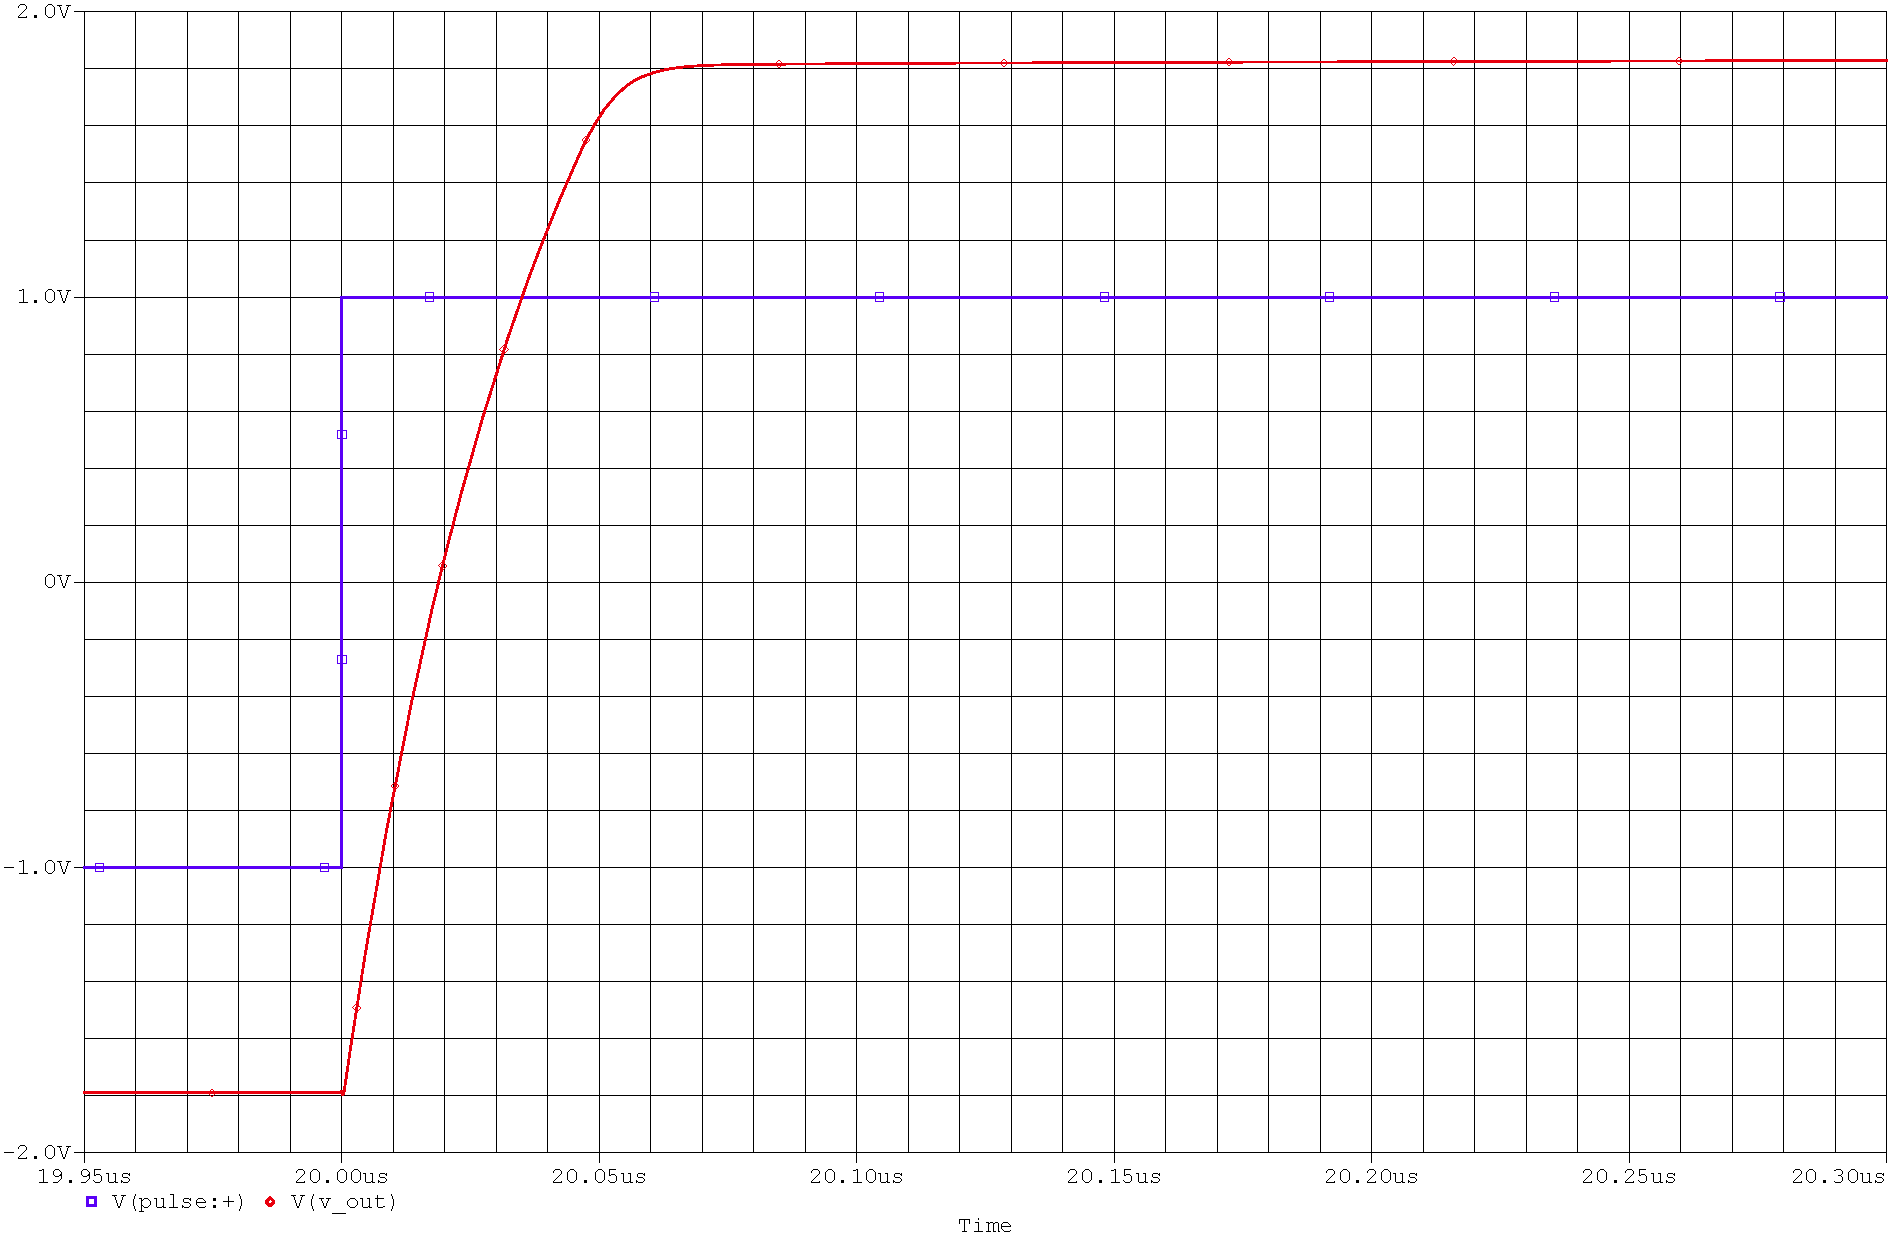
\includegraphics[width=\linewidth]{op_amp_sim/slew_rate.pdf}
		\caption{Με κόκκινο χρώμα διαγράφεται η έξοδος του τελεστικού ενισχυτή και με μπλε χρώμα διαγράφεται ο τετραγωνικός παλμός πλάτους $1\unit{\volt}$ που εφαρμόζεται στην μη αναστρέφουσα είσοδό του.}
		\label{plot:slew_rate}
	\end{plotenv}
\end{center}

% \vspace*{-0.5cm}
\subsection{Temperature sweep}

Όλες οι παραπάνω προσομοιώσεις επαναλήφθηκαν σε θερμοκρασίες $-20\unit{\celsius}$, $0\unit{\celsius}$, $20\unit{\celsius}$, $40\unit{\celsius}$, $60\unit{\celsius}$, $80\unit{\celsius}$ και $100\unit{\celsius}$. Στον πίνακα \ref{table:measurements_temp} δίνονται οι μετρήσεις των κυματομορφών. Η κατανάλωση ισχύος βρέθηκε μέσω των output αρχείων των παραμετρικών προσομοιώσεων.\par

\begin{table}[H]
	\begin{center}
		\footnotesize{\begin{tabular}{|r|c|c|c|c|}
				\hline
				\textbf{Μέγεθος}                                 & $\mathbf{-20\unit{\celsius}}$ & $\mathbf{0\unit{\celsius}}$ & $\mathbf{20\unit{\celsius}}$ & $\mathbf{27\unit{\celsius}}$ \\\hline\hline
				$20\cdot\log_{10}{\(A_v\)}\;[\unit{\decibel}]$   & $25.53643$                    & $25.54701$                  & $25.55431$                   & $25.55619$                   \\\hline
				$\mathrm{GB}\;[\unit{\mega\hertz}]$              & $10.51383$                    & $9.67467$                   & $8.93937$                    & $8.70313$                    \\\hline
				$\phi_M$                                         & $59.09589^\circ$              & $59.46750^\circ$            & $59.83206^\circ$             & $59.95727^\circ$             \\\hline
				$P_{\mathrm{diss}}\;[\unit{\milli\watt}]$        & $0.944$                       & $0.936$                     & $0.930$                      & $0.928$                      \\\hline
				$\mathrm{SR}\;[\unit{\volt\per{\micro\second}}]$ & $70.59513$                    & $69.69387$                  & $68.93170$                   & $69.20035$                   \\\hline
			\end{tabular}}
		\end{center}

		\begin{center}
		\footnotesize{\begin{tabular}{|r|c|c|c|c|}
				\hline
				\textbf{Μέγεθος}                                 & $\mathbf{40\unit{\celsius}}$ & $\mathbf{60\unit{\celsius}}$ & $\mathbf{80\unit{\celsius}}$             & $\mathbf{100\unit{\celsius}}$            \\\hline\hline
				$20\cdot\log_{10}{\(A_v\)}\;[\unit{\decibel}]$   & $25.55887$                   & $25.56106$                   & $28.67671$                               & $28.70726$                               \\\hline
				$\mathrm{GB}\;[\unit{\mega\hertz}]$              & $8.29010$                    & $7.71244$                    & \textcolor{IndianRed2}{$6.15171$}        & \textcolor{IndianRed2}{$5.65827$}        \\\hline
				$\phi_M$                                         & $60.18563^\circ$             & $60.52578^\circ$             & \textcolor{IndianRed2}{$44.59798^\circ$} & \textcolor{IndianRed2}{$44.73339^\circ$} \\\hline
				$P_{\mathrm{diss}}\;[\unit{\milli\watt}]$        & $0.924$                      & $0.920$                      & $0.916$                                  & $0.913$                                  \\\hline
				$\mathrm{SR}\;[\unit{\volt\per{\micro\second}}]$ & $68.69967$                   & $67.64329$                   & $67.17787$                               & $66.42879$                               \\\hline
			\end{tabular}}
		\end{center}
		\centering
		\caption{Μετρήσεις των παραμέτρων των προδιαγραφών για τις θερμοκρασίες $-20\unit{\celsius}$, $0\unit{\celsius}$, $20\unit{\celsius}$ και $27\unit{\celsius}$.}
		\label{table:measurements_temp}
\end{table}

Από τα δεδομένα του πίνακα \ref{table:measurements_temp} φαίνεται πως στους $80\unit{\celsius}$ και $100\unit{\celsius}$ το $\mathrm{GB}$ είναι σημαντικά χαμηλότερο της προδιαγραφής ενώ το περιθώριο φάσης είναι μόλις $0.4^\circ$ και $0.3^\circ$ κάτω των $45^\circ$ αντίστοιχα.\par

\begin{plotenv}[H]
	\centering
	\begin{tikzpicture}
		\begin{axis}[
				height=5cm,
				width=\linewidth,
				xlabel={Temperature [$\unit{\celsius}$]},
				legend style={at={(0.032,+1.025)},anchor=south west,legend columns=3},
				ymajorgrids=true,
				xmajorgrids=true,
				grid style=dashed,
				ytick=\empty
			]
			\addplot[color=IndianRed2,mark=square,thick]
			coordinates {
					(-20,25.53643)
					(0,25.54701)
					(20,25.55431)
					(27,25.55619)
					(40,25.55887)
					(60,25.56106)
					(80,28.67671)
					(100,28.70726)
				};
			\addlegendentry{$20\cdot\log_{10}{\(A_v\)}\;[\unit{\decibel}]$}

			\addplot[color=SeaGreen3,mark=*,thick]
			coordinates {
					(-20,10.51383)
					(0,9.67467)
					(20,8.93937)
					(27,8.70313)
					(40,8.29010)
					(60,7.71244)
					(80,6.15171)
					(100,5.65827)
				};
			\addlegendentry{$\mathrm{GB}\;[\unit{\mega\hertz}]$}

			\addplot[color=SlateBlue3,mark=triangle,thick]
			coordinates {
					(-20,59.09589)
					(0,59.46750)
					(20,59.83206)
					(27,59.95727)
					(40,60.18563)
					(60,60.52578)
					(80,44.59798)
					(100,44.73339)
				};
			\addlegendentry{$\phi_M$}

			\addplot[color=Turquoise4,mark=diamond,thick]
			coordinates {
					(-20,0.944)
					(0,0.936)
					(20,0.930)
					(27,0.928)
					(40,0.924)
					(60,0.920)
					(80,0.916)
					(100,0.913)
				};
			\addlegendentry{$P_{\mathrm{diss}}\;[\unit{\milli\watt}]$}

			\addplot[color=PaleVioletRed3,mark=pentagon,thick]
			coordinates {
					(-20,70.59513)
					(0,69.69387)
					(20,68.93170)
					(27,69.20035)
					(40,68.69967)
					(60,67.64329)
					(80,67.17787)
					(100,66.42879)
				};
			\addlegendentry{$\mathrm{SR}\;[\unit{\volt\per{\micro\second}}]$}
		\end{axis}
	\end{tikzpicture}
	\caption{Ποιοτική μεταβολλή των παραμέτρων $A_v$, $\mathrm{GB}$, $\phi_M$, $P_\mathrm{diss}$ και $\mathrm{SR}$ συναρτήσει της θερμοκρασίας.}
	\label{plot:parameter_temp}
\end{plotenv}

Από τα δεδομένα του πίνακα \ref{table:measurements_temp} και το διάγραμμα \ref{plot:parameter_temp} παρατηρείται πως τα μόνα μεγέθη με γνησίως καθοδική πορεία είναι το slew rate και το gain-bandwidth product.\par
Το gain-bandwidth product παρουσιάζει μία σχεδόν γραμμική μείωση με την αύξηση της θερμοκρασίας. Στους $80\unit{\celsius}$ βγαίνει εκτός προδιαγραφών κατά περίπου $1\unit{\mega\hertz}$.\par
Στην κατανάλωση ισχύος, παρατηρείται μία μικρή αύξηση με την άνοδο της θερμοκρασίας και η διαφορά μεταξύ των $-20\unit{\celsius}$ και των $100\unit{\celsius}$ είναι $31\unit{\micro\watt}$.\par
Ενδιαφέρον παρουσιάζει η απότομη και μεγάλη πτώση του περιθωρίου φάσης, $\phi_M$ μετά τους $60\unit{\celsius}$. Από $-20\unit{\celsius}$ έως και $60\unit{\celsius}$ αυξάνεται σχεδόν γραμμικά. Έπειτα, από τους $80\unit{\celsius}$ προς τους $100\unit{\celsius}$ παρατηρείται μία αρκετά μικρή αλλά αισθητή αύξηση.\par
Το κέρδος παραμένει σχεδόν σταθερό έως και τους $60\unit{\celsius}$. Αυξάνεται στους $80\unit{\celsius}$ κι έπειτα παραμένει σχεδόν σταθερό.\par